
\normalfont

En este método, utilizamos las tablas de alineaciones según el apunte de la cátedra, figura~\figref{fig:align_modes_table}. \\
Para este caso, el $Q_{T} = 0.303$ según la consigna. Por lo tanto observando la tabla, podemos tomar las columnas que indican el valor de los cocientes entre frecuencia de corte sobre frecuencia de resonancia al aire, $\left( \frac{f_{3}}{f_{s}} \right)$, frecuencia de corte sobre frecuencia de sintonía de la caja, $\left( \frac{f_{3}}{f_{b}} \right)$ y relación con complianzas, $\left( \frac{C_{as}}{C_{ab}} \right)$. \\


\begin{figure}[H]
	\centering
	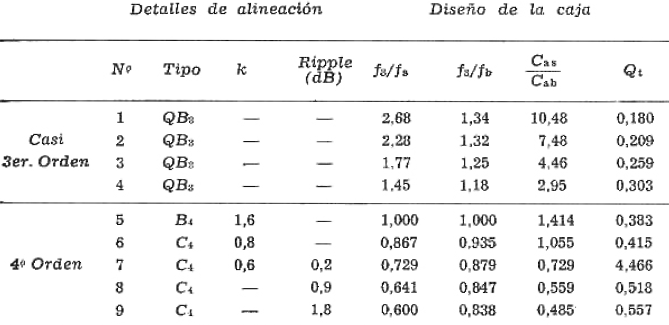
\includegraphics[width=1\textwidth]{./img/diag/align_modes.png}
	\caption{Modos de alineación de reflectores graves.}
	\label{fig:align_modes_table}
\end{figure}


Se despejan los valores de $f_{3}$ y $f_{b}$ de las relaciones obtenidas de la tabla.


\begin{equation}
\frac{f_{3}}{f_{s}} = 1.45
\end{equation}


\begin{equation}
\frac{f_{3}}{f_{b}} = 1.18
\end{equation}

Se obtiene:

\begin{equation*}
\mathcolorbox{EQColor}{ f_{3_{TS}} = 26.1 \si[per-mode=symbol]{\hertz} }
\end{equation*}


\begin{equation*}
\mathcolorbox{EQColor}{ f_{b_{TS}} = 22.12 \si[per-mode=symbol]{\hertz} }
\end{equation*}


\clearpage


El volumen del gabinete queda definido por la siguiente relación:

\begin{equation}
\frac{C_{as}}{C_{ab}} = \frac{V_{as}}{V_{box}}
\end{equation}

Se obtiene:

\begin{equation*}
\mathcolorbox{EQColor}{ V_{box_{TS}} = 69.118 \si[per-mode=symbol]{\liter} }
\end{equation*}




%% \noindent
%% \begin{center}
 
%%\begin{spacing}{1}  
\begin{table}[H]  %%\centering

    \setlength\arrayrulewidth{1.5pt}
    \arrayrulecolor{white}
    \def\clinecolor{\hhline{|>{\arrayrulecolor{white}}-%
    >{\arrayrulecolor{white}}|-|-|-|}}
\resizebox{0.98 \textwidth}{!}{% 
       
\begin{tabularx}{1 \textwidth}%
    {|
    >{\columncolor{white} \centering\arraybackslash}m{0.20\textwidth}
     |
    >{\columncolor{white} \centering\arraybackslash}m{0.35\textwidth}
     |
    >{\columncolor{white} \centering\arraybackslash}m{0.45\textwidth}
     |
    }
    \rowcolor{EQColor} \thead{Parámetro}  & \thead{Recomendado} & \thead{Diseñado} \\    
    \hhline{|-|-|-|}
    \rowcolor{gray!20} \cellcolor{gray!40} $V_{box}$ &  $129 \si[per-mode=symbol]{\liter}$ & $69.118 \si[per-mode=symbol]{\liter}$ \\  
    \hhline{|-|-|-|}  
    \rowcolor{gray!20} \cellcolor{gray!40} $f_{3}$ & $21 \si[per-mode=symbol]{\hertz}$ & $26.1 \si[per-mode=symbol]{\hertz}$ \\
    \hhline{|-|-|-|}  
    \rowcolor{gray!20} \cellcolor{gray!40} $f_{b}$ & $20 \si[per-mode=symbol]{\hertz}$ & $22.12 \si[per-mode=symbol]{\hertz}$ \\  
    \end{tabularx}}
	\caption{\footnotesize{Comparación de los valores diseñados (\textit{Thiele-Small}) con los recomendados por el fabricante.}}
	\label{table:table_comparison_TS_recomendations}
\end{table}
%%\end{spacing}

Con los valores diseñados, recordando que tiene que contener el parlante de $32 \si[per-mode=symbol]{\centi\meter}$ de diámetro y $15 \si[per-mode=symbol]{\centi\meter}$ de largo, podemos calcular las dimensiones de la caja.

Si hacemos el largo de $33 \si[per-mode=symbol]{\centi\meter}$ para acomodar el diámetro del parlante, y redondeando el volumen obtenido a $69200 \si[per-mode=symbol]{\cubic\centi\meter}$, haciendo la base cuadrada obtenemos:


\begin{equation*}
Alto = Ancho = \sqrt{\frac{V_{box}}{Largo}} = \sqrt{\frac{69200 \si[per-mode=symbol]{\cubic\centi\meter}}{33 \si[per-mode=symbol]{\centi\meter}}} = 45.80 \si[per-mode=symbol]{\centi\meter} \approx 46 \si[per-mode=symbol]{\centi\meter}
\end{equation*}

Finalemente obtenemos:


\begin{mymathbox}[ams align*, title=Dimensiones de la caja (método de \textit{Thiele-Small}), colframe=EQColor!30!EQColor]
Alto = 46 \si[per-mode=symbol]{\cubic\centi\meter} \\
Ancho = 46\si[per-mode=symbol]{\cubic\centi\meter} \\
Largo = 33 \si[per-mode=symbol]{\cubic\centi\meter}
\end{mymathbox}



